\documentclass[a4paper,11pt]{article}
\usepackage[utf8]{inputenc}
\usepackage{lastpage}
\usepackage{fancyhdr}
\usepackage[english]{babel}
\usepackage[a4paper,margin=1in]{geometry}
\usepackage{multirow}
\usepackage[table,xcdraw]{xcolor}
\usepackage{array}
\usepackage{graphicx}
\usepackage{caption}
\usepackage{ctable}
\usepackage{listings}
\usepackage[T1]{fontenc}
\usepackage{bigfoot} % to allow verbatim in footnote
\usepackage[numbered,framed]{matlab-prettifier}
\usepackage{amsmath}


\newcolumntype{L}[1]{>{\raggedright\let\newline\\\arraybackslash\hspace{0pt}}m{#1}}
\newcolumntype{C}[1]{>{\centering\let\newline\\\arraybackslash\hspace{0pt}}m{#1}}
\newcolumntype{R}[1]{>{\raggedleft\let\newline\\\arraybackslash\hspace{0pt}}m{#1}}

\newcommand\tab[1][4mm]{\hspace*{#1}}


%-------------------------------------------------------------------------------
% HEADER & FOOTER
%-------------------------------------------------------------------------------

\pagestyle{fancy}
\fancyhf{}
\setlength\headheight{15pt}
\fancyhead[L]{ Imaging Lab 7 }
\fancyhead[R]{Student ID: 100633486}
\fancyfoot[R]{Page \thepage\ of \pageref{LastPage}}


%-------------------------------------------------------------------------------
% TITLE PAGE
%-------------------------------------------------------------------------------

\begin{document}

\title{
	\Huge \textbf {Total Variation Denoising}
    \\ [0.2cm]
	\LARGE Imaging Lab 7 - May, 2017
    \\ [0.5cm]
    \hrule
}

\date{}

\author{
		\Large Kamyar Nazeri \\
		\large Student ID: 100633486 }

\maketitle
\newpage

\section*{Total Variation Denoising: Color Images}
The Rudin-Osher-Fatemi Total Variation (TV) Energy is the most famous and widely used image restoration model and for an input image \emph{f} is defined as:
\begin{align*}
\boldsymbol{min\ E_{TV}[u|f] = \int\limits_{\Omega} \Vert\nabla u\Vert d\vec{x} + \lambda \int\limits_{\Omega} (u-f)^2 d\vec{x}}
\end{align*}
Where \emph{f} is the original noisy image and $\lambda$ is parameter (fidelity weight) that controls the relative importance of the terms.
According to \emph{Lagrange-Euler} equation, the first variation of energy of this function is:
\begin{align*}
\nabla E = -\nabla \cdot \bigg(\frac{\nabla u}{\Vert\nabla u\Vert}\bigg) + 2\lambda(u-f)
\end{align*}
Where
\begin{align*}
\Vert\nabla u\Vert = \sqrt{u_x^2 + u_y^2}
\end{align*}
\\The energy is convex, so we can use steepest descent to evolve the PDE:
\begin{align*}
\frac{\partial u}{\partial t} = \frac{u_{xx} u_y^2 - 2 u_x u_y u_{xy} + u_{yy} u_x^2}{(u_x^2 + u_y^2)^{3/2}} - 2 \lambda(u-f)
\end{align*}
 \\
To apply TV denoising on a color image, we calculate the equation above on each of the 3 RGB channels and storing it in the corresponding channel of a new image. As the first step inside the for loop, we calculate the central differences to approximate the first
derivatives $u_x$ and $u_y$:
\begin{align*}
u_x \approx D_x^{0}u = \big(u(x+1,y)-u(x-1,y)\big)/2 \\
u_y \approx D_y^{0}u = \big(u(x,y+1)-u(x,y-1)\big)/2 \\
\end{align*}
And to calculate $u_{xx}$ and $u_{yy}$ we perform central differences twice on the input image; to calculate $u_{xy}$ we use diagonal derivative:
\begin{flalign*}
u_{xx} \approx D_x^{0}(D_x^{0}u) &= u(x+1,y)-2u(x,y)+u(x-1,y) \\
u_{yy} \approx D_y^{0}(D_y^{0}u) &= u(x,y+1)-2u(x,y)+u(x,y-1) \\
u_{xy} \approx D_x^{0}(D_y^{0}u) &= u(x+1,y+1)+u(x-1,y-1)-u(x-1,y+1)-u(x+1,y-1) \\
\end{flalign*}
Finally the PDE becomes:
\begin{align*}
u^{n+1} = u^n + \Delta t\ \bigg[\frac{u_{xx} u_y^2 - 2 u_x u_y u_{xy} + u_{yy} u_x^2}{(u_x^2 + u_y^2)^{3/2}} - 2 \lambda(u-f)\bigg]
\end{align*}
\\We use Forward Euler Method with Neumann boundary conditions to solve the above equation.

\newpage
\section*{Coding Total Variation on Color Images}
\emph{Listing 1} shows the  Total Variation denoising applied on a grayscale image in Matlab; \emph{Listing 2} uses the same function to apply TV on color images, and calculates SNR/RMSE of the output:
\begin{lstlisting}[caption={Total Variation function on grayscale images in Matlab},captionpos=b,style=Matlab-editor]
function [u] = tv(f, lambda)
    % Computes the total variation of an input grayscale image

    dt = 0.1;               % time step
    T = 20;                 % stopping time
    a = 0.1;                % fudge factor
    [m,n] = size(f);        % image size
    f = double(f);          % convert to double
    u = f;                  % initialization

    for t = 0:dt:T
        % u_x = (u(x+1,y) - u(x-1,y)) / 2
        u_x = (u(:,[2:n,n]) - u(:,[1,1:n-1])) / 2;

        % u_y = (u(x,y+1) - u(x,y+1)) / 2
        u_y = (u([2:m,m],:) - u([1,1:m-1],:)) / 2;

        % u_xx = u(x+1,y) - 2u(x,y) + u(x-1,y)
        u_xx = u(:,[2:n,n]) - 2 * u + u(:,[1,1:n-1]);

        % u_yy = u(x,y+1) - 2u(x,y) + u(x,y-1)
        u_yy = u([2:m,m],:) - 2 * u + u([1,1:m-1],:);

        % u_xy = (u(x+1,y+1) + u(x-1,y-1) - u(x-1,y+1) - u(x+1,y-1)) / 4
        u_xy = (u([2:m,m],[2:n,n]) + u([1,1:m-1],[1,1:n-1]) - u([2:m,m],[1,1:n-1]) - u([1,1:m-1],[2:n,n])) / 4;

        k_num = (u_xx.*u_y.^2)-2*(u_x.*u_y.*u_xy)+(u_yy.*u_x.^2);
        k_denom = (u_x.^2 + u_y.^2).^(3/2) + a;
        pde = k_num ./ k_denom - 2 * lambda * (u - f);

        u = u + dt * pde;
    end

    u = uint8(u);
end

\end{lstlisting}

\begin{lstlisting}[caption={Total Variation + RMSE/SNR on color images in Matlab},captionpos=b,style=Matlab-editor]
function [u, snr, rmse] = colortv(f, lambda)
    u = f;
    for i=1:3; u(:,:,i) = tv(f(:,:,i), lambda); end;
    snr = SNR(rgb2gray(f), rgb2gray(u));
    rmse = RMSE(rgb2gray(f), rgb2gray(u));
end
\end{lstlisting}

\newpage

\emph{Figure 1} shows a test image and three TV donoised images for different values of fidelity weight parameter. As shown below, when fidelity weight is too small the output image becomes blurry; on contrast when fidelity weight is too large, the output image resembles the original noisy input image:

\begin{figure}[!htb]
  \centering
  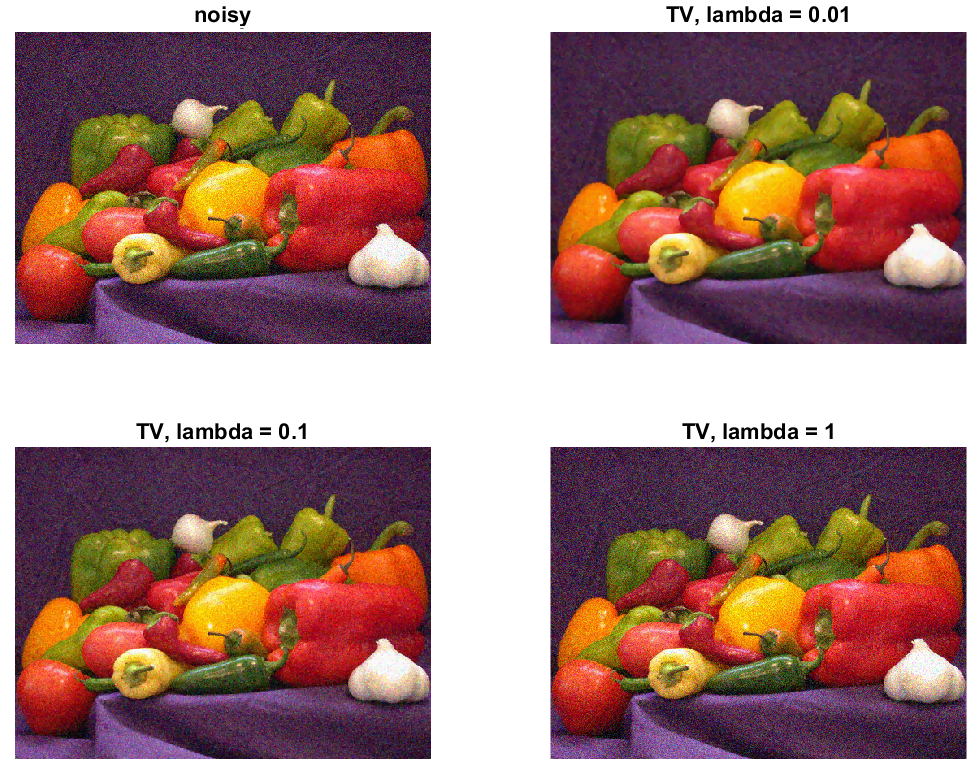
\includegraphics[width=16cm, height=12.6cm]{1.png}
  \caption{\small Total Variation denoising applied on a color image with different fidelity weight values.}
\end{figure}

\end{document}
